\chapter{Research Proposal}
\label{ch:proposal}

Experimental Design

\section{Experiment Preparations}
\label{sec:prep}

Diff sims (SFCOMPO space represented bc this offers better real-world testing for more technologies)
The next step is to provide a larger, more diverse training set to the
algorithms so they could predict better when faced with new instances.  Dayman
training/test set -> sfcompo-like sims and testing set

To obtain reliable models, one must both choose or create a training set
carefully and study the impact of various algorithm parameters on the error.
Many algorithms are developed on an assumption that the training set will be \gls{i.i.d.}.
This is important so that the
model does not overvalue or overfit a certain area in the training space. 



\section[Experiment 1: Direct Isotopics]{Experiment 1\\ {\textit{Viability of Statistical Learning on Direct Isotopics}}}
\label{sec:exp1}

\begin{figure}[!htb]
    \centering
    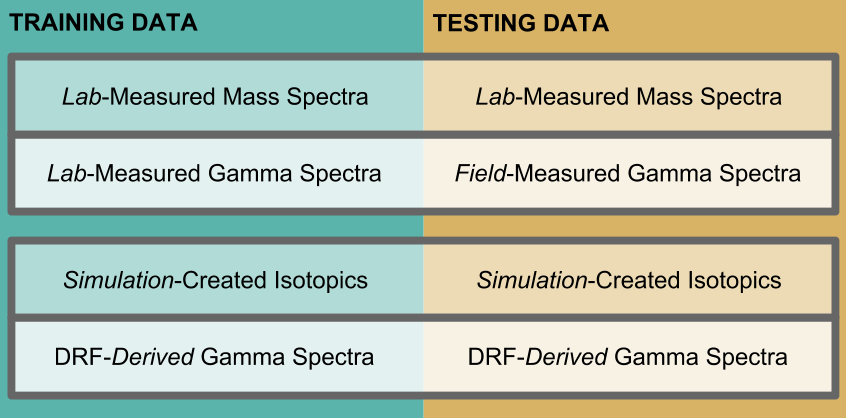
\includegraphics[width=\linewidth]{./chapters/proposal/proposal.png}
    \caption{Basis for Experiments 1 and 2.}
    \label{fig:proposal}
\end{figure}


\section[Experiment 2: Gamma Spectra]{Experiment 2\\ {\textit{Viability of Statistical Learning on Gamma Spectra}}}
\label{sec:exp2}

hey

\section[Experiment 3: Other Fuel Cycle Flows]{Experiment 2\\ {\textit{Viability of Statistical Learning on Other Fuel Cycle Flows}}}
\label{sec:exp3}

hey
